% BEGIN STANDALONE PREVIEW PREAMBLE
% When input into a paper, its class already defines \subsection and this is skipped.
\ifdefined\subsection
\else
  \documentclass[11pt]{article}
  \usepackage[margin=20mm]{geometry}
  \usepackage{graphicx}
  \usepackage{url}
  \newcommand{\CPOSSStandalonePreview}{}
  \begin{document}
\fi
% END STANDALONE PREVIEW PREAMBLE

\subsection{Chemical composition and molecular-size coverage}
We compared the chemical content of CPOSS with the training split of Open Molecular Crystals 2025 (OMC25)\cite{gharakhanyan2026omc25}, counting each documented CPOSS molecular system and each OMC25 CSD reference code once (Fig.~\ref{fig:cposs_omc25_comparison}). The principal comparison contains 190 single-component CPOSS systems with coordinate-validated compositions and 44,403 OMC25 molecular records. Repeated CSP searches, energy models, generated packings and relaxation frames do not weight these molecular distributions. A further 44 CPOSS multicomponent systems are described separately on their complete stoichiometric formula-unit basis. One CPOSS system with no valid alternative coordinate element table was excluded from the coordinate-validated population; including the reported formula gives a supplementary metadata-only population of 191 single-component systems.

CPOSS single-component systems contain 5--100 atoms per molecule (median 18), compared with 4--164 atoms (median 39) in OMC25. The corresponding median non-hydrogen atom counts are 12 and 21. Using one average-atomic-weight convention for both datasets, CPOSS molar masses span 32.04--890.88\,g\,mol$^{-1}$ (median 179.69\,g\,mol$^{-1}$), whereas OMC25 spans 30.03--1386.32\,g\,mol$^{-1}$ (median 312.15\,g\,mol$^{-1}$). These summaries describe the observed molecular populations and do not establish equivalence of their chemical environments or crystal packings.

Elemental occurrence is expressed as the fraction of molecular records containing each species. Oxygen occurs in 78.9\% of CPOSS systems and 81.9\% of OMC25 molecular records, while nitrogen occurs in 71.6\% and 65.4\%, respectively. The verified CPOSS population also contains Cu, outside the elemental vocabulary of OMC25. Its occurrence does not imply that OMC25 models have been evaluated on this chemistry. CPOSS additionally includes salts, solvates and co-crystals, which require a distinct formula-unit basis and are outside OMC25's stated single-component scope. The comparison therefore describes complementary sampling priorities: repeated crystal-energy-landscape searches in CPOSS and broad molecular sampling for training interatomic potentials in OMC25. The supplied reference figure provides no CSD elemental, molecular-size or mass distributions, so no such CSD curves are inferred here.

% BEGIN DENSITY COMPARISON
\subsection{Crystal-density distributions}
We compared CPOSS crystal densities with the OMC25 last-frame and organic CSD 6.00 reference histograms in Fig.~3a of the OMC25 paper\cite{gharakhanyan2026omc25} (Fig.~\ref{fig:cposs_omc25_csd_density}). The CPOSS density population comprises 114,222 archive-linked visualisation records from 257 searches covering 186 single-component molecular systems. For each search, we selected the lowest-numbered archived energy model with an unambiguous density column labelled in g\,cm$^{-3}$, retained finite positive values whose filenames match that archive, and counted repeated filenames once per search. These are source-reported densities from the visualised subset, rather than a complete density census of all archived CPOSS files. Experimental-match annotations were retained because they also label predicted structures; the records are not claimed to be geometrically unique minima.

The OMC25 and CSD bar heights were recovered from the vector graphic and therefore provide approximate binned references rather than raw per-crystal measurements. Their different original bin widths were accounted for by conservative overlap rebinning to 0.02\,g\,cm$^{-3}$ bins. All curves were normalised within the common displayed interval 0.8--2.4\,g\,cm$^{-3}$; 0.89\% of the available CPOSS single-component records fall outside this interval and are reported separately. Within this interval, the CPOSS record-weighted median density is 1.35\,g\,cm$^{-3}$, compared with approximately 1.29\,g\,cm$^{-3}$ for OMC25 and 1.34\,g\,cm$^{-3}$ for the CSD reference. Giving each CPOSS molecular system equal weight, with equal weights for its searches, changes its conditional median to 1.38\,g\,cm$^{-3}$. This sensitivity reflects the unequal numbers of stored crystal candidates across CPOSS landscapes. Density agreement is descriptive and does not establish agreement in chemical composition, packing motifs or relative stability; the CSD reference contains experimentally determined crystals, whereas the computational populations also depend on their generation, relaxation and selection procedures.
% END DENSITY COMPARISON

% BEGIN STANDALONE PREVIEW FOOTER
% Only the editor's standalone preview includes these figures and reference.
\ifdefined\CPOSSStandalonePreview
  \begin{figure}[p]
    \centering
    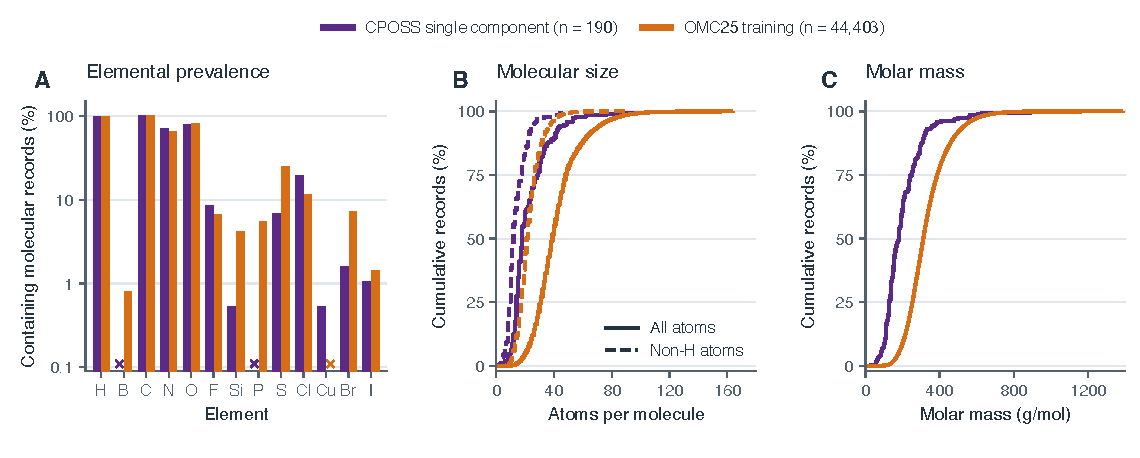
\includegraphics[width=\textwidth]{output/pdf/cposs_omc25_comparison.pdf}
    \caption{\textbf{Chemical content of CPOSS and OMC25.} The comparison uses 189 single-component CPOSS molecular systems with compositions checked against archived coordinate representatives and 44,403 molecular records from the OMC25 training split. Each CPOSS system is counted once by its documented source page, and each OMC25 molecule once by its CSD reference code after verifying invariant molecular metadata across its starting-crystal records. Records are not merged by molecular formula. Repeated searches, energy models, crystal packings and relaxation frames do not weight the distributions. \textbf{(A)} Percentage of molecular records containing each element, using the union of species present in either dataset. Categories overlap and need not sum to 100\%. The ordinate is logarithmic; crosses at the lower edge denote zero occurrence. \textbf{(B)} Empirical cumulative distributions of molecular atom counts, including all hydrogens (solid) or excluding hydrogen (dashed). \textbf{(C)} Empirical cumulative distributions of molar mass, calculated from complete molecular compositions using the same frozen RDKit average atomic weights for both datasets. Official OMC25 \texttt{mol.mass} values are retained in the data tables; harmonisation changes individual training-set masses by at most 0.032\,g\,mol$^{-1}$. All ECDFs are evaluated without binning. The source audit's eight composition conflicts and two malformed website formulas were reviewed against workbook and coordinate evidence, with all source choices recorded. One CPOSS system with no valid alternative coordinate element table was excluded from the primary comparison and retained in a separate metadata-only sensitivity analysis. The 44 verified multicomponent CPOSS systems are shown separately in the supplementary comparison using complete written stoichiometry or explicitly documented coordinate-derived component ratios. OMC25's molecular basis follows its published single-component definition; connectivity was not independently reconstructed from its metadata CSV. These molecular distributions do not describe unit-cell sizes or counts of independent crystal minima.}
\label{fig:cposs_omc25_comparison}

  \end{figure}
  \begin{figure}[p]
    \centering
    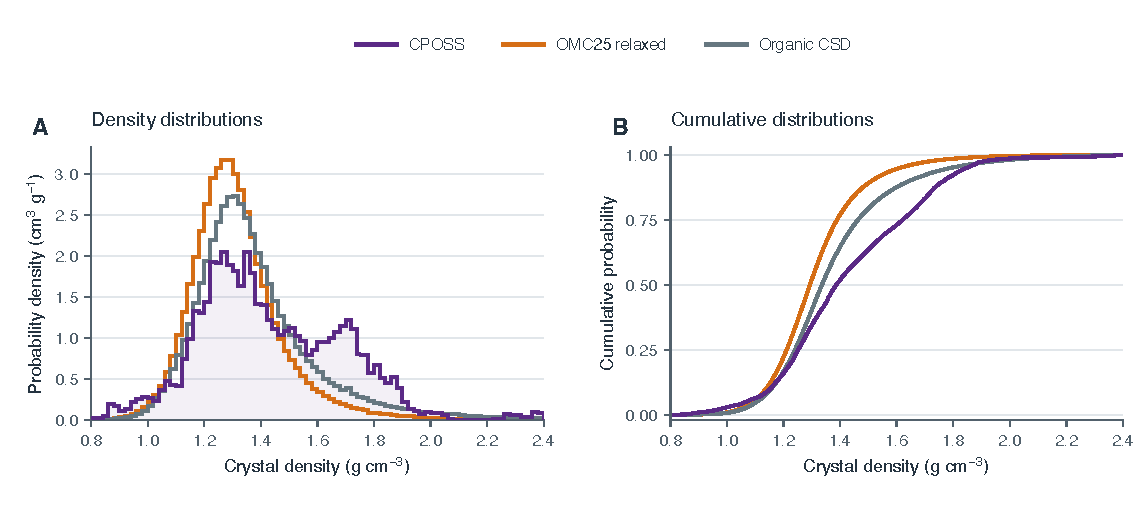
\includegraphics[width=\textwidth]{output/pdf/cposs_omc25_csd_density_comparison.pdf}
    \caption{\textbf{Crystal-density distributions in CPOSS, OMC25 and the CSD.} \textbf{(A)} Normalised histograms of source-reported CPOSS densities and the OMC25 last-relaxation-frame and organic CSD 6.00 references recovered from Fig.~3a of the OMC25 paper\cite{gharakhanyan2026omc25}. The CPOSS sample contains 114,222 archive-linked visualisation records from 257 searches and 186 single-component molecular systems. Each search contributes the lowest-numbered archived energy model with a uniquely matched density column in g\,cm$^{-3}$; only finite positive densities whose filenames occur in that archive are retained, and repeated filenames are counted once per search. No geometric deduplication across searches is implied. Experimental-match annotations are retained because they can describe predicted structures. The CPOSS values describe the available visualisation subset, rather than all archived structure files. Reference bar heights are recovered from the paper's vector graphic and remain approximate, with no raw CSD or OMC25 per-crystal densities reconstructed. The original CSD and OMC25 bin widths differ; reference count mass is redistributed by bin overlap onto common 0.02\,g\,cm$^{-3}$ bins. Every distribution is normalised independently within 0.8--2.4\,g\,cm$^{-3}$, so tails outside this interval are not compared. The excluded-window fraction is 0.89\% for the available CPOSS single-component records. \textbf{(B)} Conditional cumulative distributions. CPOSS curves use the source density values; reference curves assume uniform probability within the recovered bins. The dashed CPOSS curve gives each molecular system equal total weight, then each of its searches equal weight, before conditioning on the common window. This exposes sensitivity to the uneven number of candidates in each landscape.}
\label{fig:cposs_omc25_csd_density}

  \end{figure}
  \begin{thebibliography}{1}
    \bibitem{gharakhanyan2026omc25}
    V.~Gharakhanyan et al.,
    Open Molecular Crystals 2025 (OMC25) dataset and models,
    \textit{Scientific Data} (2026).
    \url{https://doi.org/10.1038/s41597-026-06628-2}.
  \end{thebibliography}
  \end{document}
\fi
% END STANDALONE PREVIEW FOOTER
